\documentclass[12pt, oneside, final]{report}
\usepackage{geometry}
\geometry{a4paper, left=20mm, right=20mm, top=25mm, bottom=25mm}
\usepackage[utf8]{inputenc}
\usepackage{t1enc}
\usepackage[MeX]{polski}
\usepackage{graphicx}
\usepackage{amsmath}
\usepackage{amssymb}
\usepackage{mathtools}
\usepackage{indentfirst}
\usepackage{pdfpages}
\usepackage{xcolor}
\usepackage{placeins} % provides \FloatBarrier
\usepackage{tikz}
\usetikzlibrary{positioning,shapes,arrows,calc,decorations.markings,shadows}
\usepackage[hidelinks]{hyperref}

% Czcionka
\usepackage{charter}

% Pojedyncze elementy na górze stron
\makeatletter
\setlength{\@fptop}{0pt}
\makeatother

% Styl tytułowania rozdziałów:
\usepackage{titlesec}
%\titleformat{\chapter}{\normalfont\huge}{\bf\thechapter.}{20pt}{\huge\bf}
% Styl tytułowania rozdziałów:
\titleformat{\chapter}[display] 
{\centering\normalfont\huge\bfseries}{\centering\chaptertitlename\ \thechapter.}{0.5em}{}
\titlespacing{\chapter}{0em}{0em}{2em}

% dodatkowe kropki po numerach rozdziałów, sekcji itd
\usepackage{titlesec}
\titlelabel{\thetitle.\quad}

% Dodatkowe odstępy w tabelach
\usepackage{array}
\setlength\extrarowheight{4pt}

% Wyłączone wcięcia
\usepackage{parskip}

\begin{document}
% Title page
\begin{titlepage}
	\centering
	\begin{figure}
		\centering
		
\includegraphics[width=0.9\textwidth]{logo.pdf}
	\end{figure}
	\vspace*{100pt}
	\LARGE{Podstawy Sztucznej Inteligencji}\\
	\vspace{30pt}
	\textsc{\Huge{Projekt WG.AE.1}}\\
	\vspace{120pt}
	\Large{Marcin Baran \textit{259804}}\\
	\Large{Łukasz Kilaszewski \textit{259822}}\\
	\Large{Mateusz Perciński \textit{Z59827}}\\
	\vfill
	\large{13 czerwca 2017}
\end{titlepage}

\thispagestyle{empty}
\tableofcontents
%\cleardoublepage

\section*{Treść zadania}
\textbf{WG.AE1 Rozwożenie mebli} \\
Zaplanować trasę samochodu ciężarowego rozwożącego meble. Każdy mebel ma określoną
wagę oraz miasto przeznaczenia. Zużycie paliwa przez samochód ciężarowy jest zależne od
masy przewożonego ładunku. Zaplanować trasą rozwiezienia mebli która jest optymalna ze
względu na zużycie paliwa. Program powinien na bieżąco prezentować jakość znalezionego
rozwiązania w funkcji numeru pokolenia.
\section*{Podział pracy}
Marcin Baran - Definicja zadania\\
Łukasz Kilaszewski - Implementacja programu\\
Mateusz Perciński - Raport oraz wnioski


\chapter{Definicja problemu}
Projekt polega na rozwiązaniu zmodyfikowanego zadania komiwojażera. Optymalizowana jest trasa (kolejność odwiedzonych miast) ciężarówki rozwożącej meble ze względu na zużycie paliwa. Na podstawie treści zadnia przyjęto, że dla każdego miasta na planowanej trasie, znana jest masa mebli, które mają być do niego dostarczone, a zużycie paliwa jest zależne masy przewożonego towaru. W kolejnych podpunktach opisano przyjęte założenia, które nie wynikają ściśle z treści zadania.

\section{Miasta}
Przyjęto, że zadanie rozwiązywane jest dla większych polskich miast, których lista wraz ze współrzędnymi geograficznymi została pobrana z %TODO 
Odległość między miastami zdefiniowana jest miarą euklidesową, jako odległość w linii prostej. Założono, że użytkownik będzie mógł wybrać miasta, mające się znaleźć na trasie przejazdu, i każdemu z nich przypisać masę mebli, które mają być w nim zostawione.

\section{Trasa}
Założenia dotyczące trasy przejazdu ciężarówki:
\begin{itemize}
\item trasa zaczyna się i kończy tym samym, określonym na początku mieście,
\item każde miasto jest odwiedzane tylko raz,
\item odległości między miastami są jednakowe w obydwu kierunkach (problem komiwojażera jest symetryczny),
\item ciężarówka zostawia w każdym mieście wszystkie, predestynowane do niego, meble. Jej masa zmniejsza się. Ostatni, powrotni odcinek, pokonywany jest bez ładunku.
\end{itemize}

\section{Zużycie paliwa}
Przyjęto, że zużycie paliwa jest wprostproporcjonalne do masy pojazdu, a w związku z tym z masą przewożonych mebli. Koszt przejazdu pomiędzy dwoma miastami, czyli zużycie paliwa na trasie między nimi, określono wzorem
\begin{equation}
cost_{section} = m_a * mass + m_b) \cdot dist,
\end{equation}
gdzie: 
\begin{description}
\item[$mass$] - masa mebli znajdujących się w ciężarówce na tym odcinku drogi,
\item[$dist$] - odległość między miastami,
\item[$m_b$] - współczynnik określający stałe spalanie ciężarówki (bez obiciążenia) $[\frac{litr}{km}]$
\item[$m_a$] - współczynnik wpływu dodatkowego obciążenia na spalanie ciężarówki $[\frac{litr}{kg \cdot km}]$
\end{description}

\section{Algorytm ewolucyjny}
Do rozwiązania problemu zastosowano algorytm ewolucyjny ($\mu$ + $\lambda$). Przyjęto, że osobnikiem jest wytyczona trasa, a jego genotypem wektor liczb całkowitych określający kolejność odwiedzanych miast. Numeracja odwiedzanych miast jest zgodna z kolejnością na liście definiującej problem (wypisującej wszystkie miasta, które mają zostać odwiedzone wraz z masami predestynowanych do nich mebli). Miasto początkowe (i jednocześnie końcowe) nie występuje w wektorze. Założono, że populacją dla algorytmu ewolucyjnego jest zbiór takich wektorów.

\subsection{Krzyżowanie}
Genotypy 2 osobników krzyżowane w następujący sposób:
\begin{itemize}
\item Losowany jest liczna będąca indeksem w wektorze kolejności miast podczas przejazdu.
\item Część wektorów znajdująca się za wylosowanym indeksem jest zamieniana między osobnikami.
\item Wybierane są geny (wartości w wektorze), które zostały odrzucone w skutek powyższych operacji oraz takie, które w się powtarzają.
\item Geny powtarzające się w ramach jednego genotypu, zostają zastąpione przez brakujące (w stosunku do pierwotnego genotypu).
\end{itemize}

\subsection{Mutacja}
Mutacja genotypu danego osobnika polega na zamianie dwóch kolejnych genów, czyli wartości w wektorze kolejności odwiedzanych miast. Wybór genu, który jest zamieniany z sąsiadem, jest dokonywany losowo.

\chapter{Implementacja}
Program rozwiązujący zdefiniowany wcześniej problem komiwojażera zaimplementowano w języku Python. Wykorzystano następujące biblioteki:
\begin{itemize}
\item \textbf{numpy} - umożliwiła korzystanie z macierzy,
\item \textbf{geopy} - wykorzystano funkcję great\_circle w celu obliczania odległości miedzy dwoma miastami znając ich współrzędne geograficzne,
\item \textbf{matplotlib} - posłużyła do generowania czytelnych wykresów.
\end{itemize}

\section{Struktura programu}
Napisany program ma strukturę modułową. Głównym celem było wyodrębnienie części odpowiedzialnej za realizację obliczeń według algorytmu ewolucyjnego od części definiującej problem do rozwiązania.

\subsection{Klasa Data}
Klasa Data zawiera wszystkie informację na temat zadania, które ma być rozwiązywane. Argumentem jej konstruktora jest nazwa pliku CSV definiującego zadanie. Po wywołaniu konstruktora miasta są numerowane oraz zapisywane w tablicy wraz z ciężarami mebli. Określane są parametry $m_a$ i $m_b$. Budowana jest również tablica przechowująca odległości między dwoma dowolnymi miastami z zadania. Klasa posiada funkcje \textbf{distance} obliczająca odległość między dwoma miastami na podstawie ich współrzędnych geograficznych, oraz funkcję \textbf{get\_random\_genotype} zwracającą permutację wektora liczb, odpowiadających miastom.
\subsection{Pliki CSV}\label{sec:csv}
Plik \textit{cities.csv} zawiera większe miasta wraz z ich współrzędnymi geograficznymi. Spośród nich należy wybierać te, które mają być odwiedzone przez ciężarówkę. Definiowanie problemu do rozwiązania polega na uzupełnianiu pliku \textit{task.csv}.

\subsection{Klasa Genotype}
Klasa Genotype reprezentuje genotyp osobnika algorytmu ewolucyjnego oraz operacje z nim związane. Konstruktor przyjmuje obiekt typu Data i zapisuje go. Klasa zawiera następujące funkcje:
\begin{itemize}
\item \textbf{display} - wyświetla genotyp oraz wartość obliczonej dla niego funkcji celu,
\item \textbf{cost} - oblicza wartość funkcji celu (w naszym przypadku koszt przejazdu ciężarówki), korzystając z funkcji \textbf{section\_cost},
\item \textbf{section\_cost} - oblicza oblicza koszt przejazdu pomiędzy dwoma miastami,
\item \textbf{cross} - krzyżuje dwa genotypy,
\item \textbf{mutate} - przeprowadza mutację genotypu.
\end{itemize}
\subsection{Klasa GenethicAlgorithm}
Klasa GenethicAlgorithm reprezentuje algorytm ewolucyjny. Jego konstruktor przyjmuje i zapisuje argument typu Data oraz definiuje pozostałe zmienne obiektu. Klasa zawiera następujące funkcje:
\begin{itemize}
\item \textbf{init} - przyjmuje argumenty \textbf{population}, \textbf{cross} i \textbf{stop\_iters}, a następnie sprawdza ich poprawność,
\item \textbf{solve} - iteracyjnie rozwiązuje  zadanie wykorzystując reguły algorytmu ewolucyjnego, w każdym kroku drukując najlepszy uzyskany wynik,
\item \textbf{print\_results} - wyświetla rezultaty działania algorytmu w postaci listy miast, w kolejności, jakie należy je odwiedzić oraz kosztu przejazdu.
\item \textbf{cross} - krzyżuje dwa genotypy,
\item \textbf{mutate} - przeprowadza mutację genotypu.
\end{itemize}

\subsection{Program main}
Program main w najprostszej wersji tworzy obiekt typu Data, jako argument podając, nazwę pliku CSV z definicją zadania. następnie tworzy obiekt typu GeneticAlgorithm, podając mu obiekt typu Data. Kolejne polecenia to wywołania funkcji obiektu typu GeneticAlgorithm: \textbf{init} definiującej paramtery algorytmu, \textbf{solve} rozwiązującej zadanie, oraz \textbf{print\_result} drukującej wyniki.

\section{Instrukcja dla użytkownika}
Tak jak napisano w sekcji \ref{sec:csv}, plik \textit{cities.csv} zawiera większe miasta wraz z ich współrzędnymi geograficznymi. Spośród nich należy wybierać te, które mają być odwiedzone przez ciężarówkę. Definiowanie problemu do rozwiązania polega na uzupełnianiu pliku \textit{task.csv}. W pierwszym wierszu znajduje się nazwa miasta startowego (i jednocześnie końcowego). Następne wiersze zawierają nazwy miast, które mają zostać odwiedzone wraz z masą mebli, które mają być do nich dostarczone. Wiersz ma format $nazwa\_miasta;masa\_mebli$. Masa mebli powinna być podana jako liczba, z przynajmniej jednym miejsce dziesiętnym np. 100.0, 123.4.

Parametry algorytmu ewolucyjnego można zdefiniować jako zmieniając wartości argumentów funkcji \textbf{init} obiektu \textbf{alg}:
\begin{itemize}
\item population - ilość osobników wybieranych do populacji w każdej iteracji algorytmu,
\item cross - ilość osobników, które mają być krzyżowane w każdym kroku iteracji algorytmu,
\item stop\_iters - ilość iteracji, po której, w przypadku braku poprawy wyniku, działanie algorytmu jest przerywane.
\end{itemize}

Po zdefiniowaniu problemu do rozwiązania oraz parametrów algorytmu, należy uruchomić plik \textit{main.py}. W oknie konsoli, będą wypisywane genotypy najlepszych osobników z populacji danej iteracji wraz z obliczoną dla nich wartością funkcji oceny, którą jest określona jako zużycie paliwa.
 Po zakończeniu działania algorytmu najlepsze wartości dla najlepszych osobników każdej iteracji prezentowane się w formie wykresu.

\chapter{Testy i osiągnięte rezultaty}

\section{Różne rozwiązania tego samego problemu}
Pierwszym testem była próba rozwiązania tego samego problemu kilkukrotnie oraz porównanie wyników. Jako miasto startowe została wybrana Bydgoszcz. Kolejne miasta, które miały znaleźć się na trasie wraz z ciężarem mebli przedstawiono w tabeli \ref{tab:same-problem-same-algorithm}.

\begin{table}[ht!]
\caption{Definicja problemu do rozwiązania w pierwszym teście}
\label{tab:same-problem-same-algorithm}
\centering
\scalebox{0.9}{
\begin{tabular}{cc}
\hline 
Miasto & Masa mebli [kg]\\
\hline
Gdańsk & 400.0 \\
Katowice & 800.0 \\
Tarnów & 200.0 \\
Łódź & 100.0 \\
Szczecin & 111.0 \\
Warszawa & 100.0 \\ 
Opole & 1.0 \\
Siedlce & 300.0 \\
Kraków & 700.0 \\
Gliwice & 100.0 \\
Poznań & 50.0 \\
Kielce & 20.0 \\
Olsztyn & 300.0 \\
Suwałki & 100.0 \\
Gdynia & 150.0 \\
\hline
\end{tabular}}
\end{table}

Algorytm uruchomiono trzykrotnie, ustalając liczność populacji w każdym kroku algorytmu na 80 osobników, ilość krzyżowanych osobników - na 30, a warunek stopu, w przypadku braku poprawy rezultatu - na 30 iteracji. Parametry $m_a$ oraz $m_b$ określono w taki sposób, że pusta ciężarówka spala średnio 10 litrów na 100 km, a każde dodatkowe 100 kg bagażu, większa spalanie o 1l. Przyjęto cenę paliwa na poziomie 5 złotych za litr. Zgodnie oczekiwaniami, algorytm, ze względu na elementy losowości, w kolejnych iteracjach uzyskiwał różne wartości najmniejszego kosztu przejazdu. Ostateczne wyniki działania algorytmu również były różne. Rozwiązania problemu zostały przedstawione w tabeli \ref{tab:results-same-algorithm}. Jak widać zaproponowana kolejność odwiedzanych miast już różna. Najlepszy rozwiązanie, czyli koszt rozwożenia mebli wynoszący 2585.71 zł, zostało znalezione przy pierwszym uruchomieniu algorytmu. Najlepsze rozwiązania dla kolejnych iteracji algorytmu przedstawiono na rysunku \ref{fig:same-problem-same-algorithm}.

\begin{table}[ht!]
\caption{Rozwiązania pierwszego test}
\label{tab:results-same-algorithm}
\centering
\begin{tabular}{llll}
\hline 
Kolejność na trasie & \multicolumn{3}{c}{Numer uruchomienia algorytmu}\\
\hline
						& 1 & 2 & 3\\
\hline
1 						& Gdańsk	& Tarnów	& Gdańsk\\
2						& Gdynia	& Kraków	& Olsztyn\\
3						& Olsztyn	& Katowice	& Kielce\\
4						& Suwałki	& Gliwice	& Tarnów\\
5						& Siedlce	& Warszawa	& Kraków\\
6						& Warszawa	& Siedlce	& Katowice\\
7						& Łódź		& Suwałki	& Gliwice\\
8						& Gliwice	& Olsztyn	& Opole\\
9						& Katowice	& Gdańsk	& Łódź\\
10						& Kraków	& Gdynia	& Warszawa\\
11						& Tarnów	& Łódź		& Siedlce\\
12						& Kielce	& Kielce	& Suwałki\\
13						& Opole		& Opole		& Gdynia\\
14						& Poznań	& Poznań	& Szczecin\\
15						& Szczecin	& Szczecin	& Poznań\\
\hline
Koszt przejazdu [zł]	& 2585.71	& 2967.03 	& 2706.77\\
\hline
\end{tabular}
\end{table}



\begin{figure}[ht!]
\centering
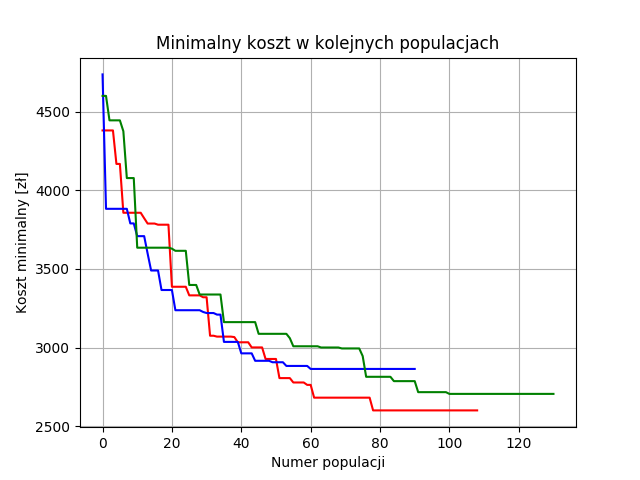
\includegraphics[width=0.7\textwidth]{graphics/same-problem-same-algorithm}
\caption{Wykres wartości najlepszego rozwiązania w kolejnych iteracjach dla 3 uruchomień tego samego algorytmu. Pierwsze uruchomienie algorytmu - kolor czerwony, drugie - niebieski, trzecie - zielony}
\label{fig:same-problem-same-algorithm}
\end{figure}

\section{Różne wielkości populacji}
W drugim teście rozwiązywano problem zdefiniowany tak, jak w teście pierwszym, zmieniano wielkość populacji w kolejnych uruchomianiach algorytmu. Przyjęto, że koniec algorytm będzie występował po 30 iteracjach bez poprawy, a ilość krzyżowanych osobników zawsze będzie stanowiła połowę populacji. Tabela \ref{tab:results-diff-population} przedstawia wyniki działania algorytmu dla 3 różnych zestawów parametrów.

\begin{table}[ht!]
\caption{Rozwiązania drugiego testu}
\label{tab:results-diff-population}
\centering
\begin{tabular}{llll}
\hline 
Kolejność na trasie & \multicolumn{3}{c}{Numer uruchomienia algorytmu}\\
\hline
						& 1 & 2 & 3\\
\hline
1 						& Katowice	& Gdańsk	& Gliwice\\
2						& Kraków	& Gdynia	& Opole\\
3						& Tarnów	& Olsztyn	& Katowice\\
4						& Siedlce	& Suwałki	& Kraków\\
5						& Olsztyn	& Siedlce	& Tarnów\\
6						& Gdańsk	& Warszawa	& Kielce\\
7						& Warszawa	& Kielce	& Łódź\\
8						& Kielce	& Tarnów	& Warszawa\\
9						& Łódź		& Kraków		& Siedlce\\
10						& Gdynia	& Katowice	& Suwałki\\
11						& Szczecin	& Gliwice		& Olsztyn\\
12						& Poznań	& Opole	& Gdańsk\\
13						& Opole		& Łódź		& Gdynia\\
14						& Gliwice	& Poznań	& Szczecin\\
15						& Suwałki	& Szczecin	& Poznań\\
\hline
Koszt przejazdu [zł]	& 3361.47	& 2538.42 	& 2673.21\\
\hline
Wielkość populacji		& 20		& 80 	& 160\\
\hline
Ilość krzyżowanych		& 10		& 40 	& 80\\
\hline

\end{tabular}
\end{table}

Wykres \ref{tab:results-diff-population} przedstawia działanie algorytmu dla podanych zestawów parametrów podanych w tabeli \ref{tab:results-diff-population}. Biorąc pod uwagę najlepsze rezultaty osiągane przez algorytmy, nie da się wyciągnąć jednoznacznego wniosku na temat jakość uzyskiwanego wyniku od wielkości populacji. Wybrane wielkości populacji były jednak bardzo małe w porównaniu ze wszystkimi możliwościami przejazdu ciężarówki (liczba rzędu $10^{12}$).

\begin{figure}[ht!]
\centering
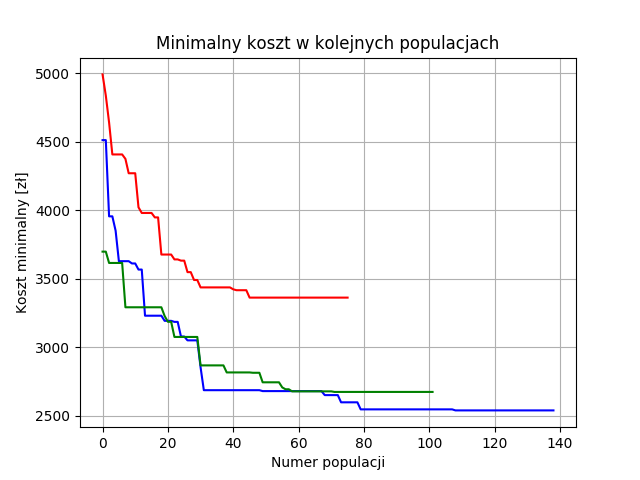
\includegraphics[width=0.7\textwidth]{graphics/diff-population}
\caption{Wykres wartości najlepszego rozwiązania w kolejnych iteracjach dla 3 uruchomień tego samego algorytmu. Pierwsze uruchomienie algorytmu - kolor czerwony, drugie - niebieski, trzecie - zielony}
\label{fig:diff-population}
\end{figure}

\section{Czas obliczeń}
 %TODO
 

\end{document}
